\section{Смешанный алгоритм глобального поиска и его эффективная реализация}
Ещё одной модификацией метода Стронгина, позволяющей в процессе оптимизации лучше учитывать данные о локальных оптимумах, найденных в процессе поиска, является смешанный алгоритм Стронгина-Маркина \cite{mixedAlg}.
Наряду с характеристикой интервала \(R(i)\) (\ref{step3_2}) можно рассматривать \(R^*(i)\), которая будет более чувствиетльна к наличию в интревале текущего найденного минимума функции \(z^*\):
\begin{displaymath}
R^*(i)=R(i)/(\sqrt{(z_i-z^*)(z_{i-1}-z^*)}/\mu + 1.5^{-\alpha})
\end{displaymath}
где \(\alpha \in [1;30]\) --- степень локальности. Чем она больше, тем более высокая характеристика у интервала, содержащего \(z^*\), по сравнению с остальными.
\par
Смешанный алгоритм состоит в следующем: в процессе работы метода каждые \(S\) итераций интервал для последующего разбиения выбирается по характеристикам \(R^*(i)\). \(S\) --- параметр смешивания.
Такой подход позволяет существенно ускорить сходимость метода. На рис. \ref{fig:localMixOP4d} приведены операционные характеристики чисто глобального и смешанного алгоритма на классе GKLS 4d Simple.
Параметр смешивания \(S=5\), остальные параметры метода были заданы такие же, как в разделе \ref{sec:multilev_maps}
\begin{figure}[ht]
	\center
  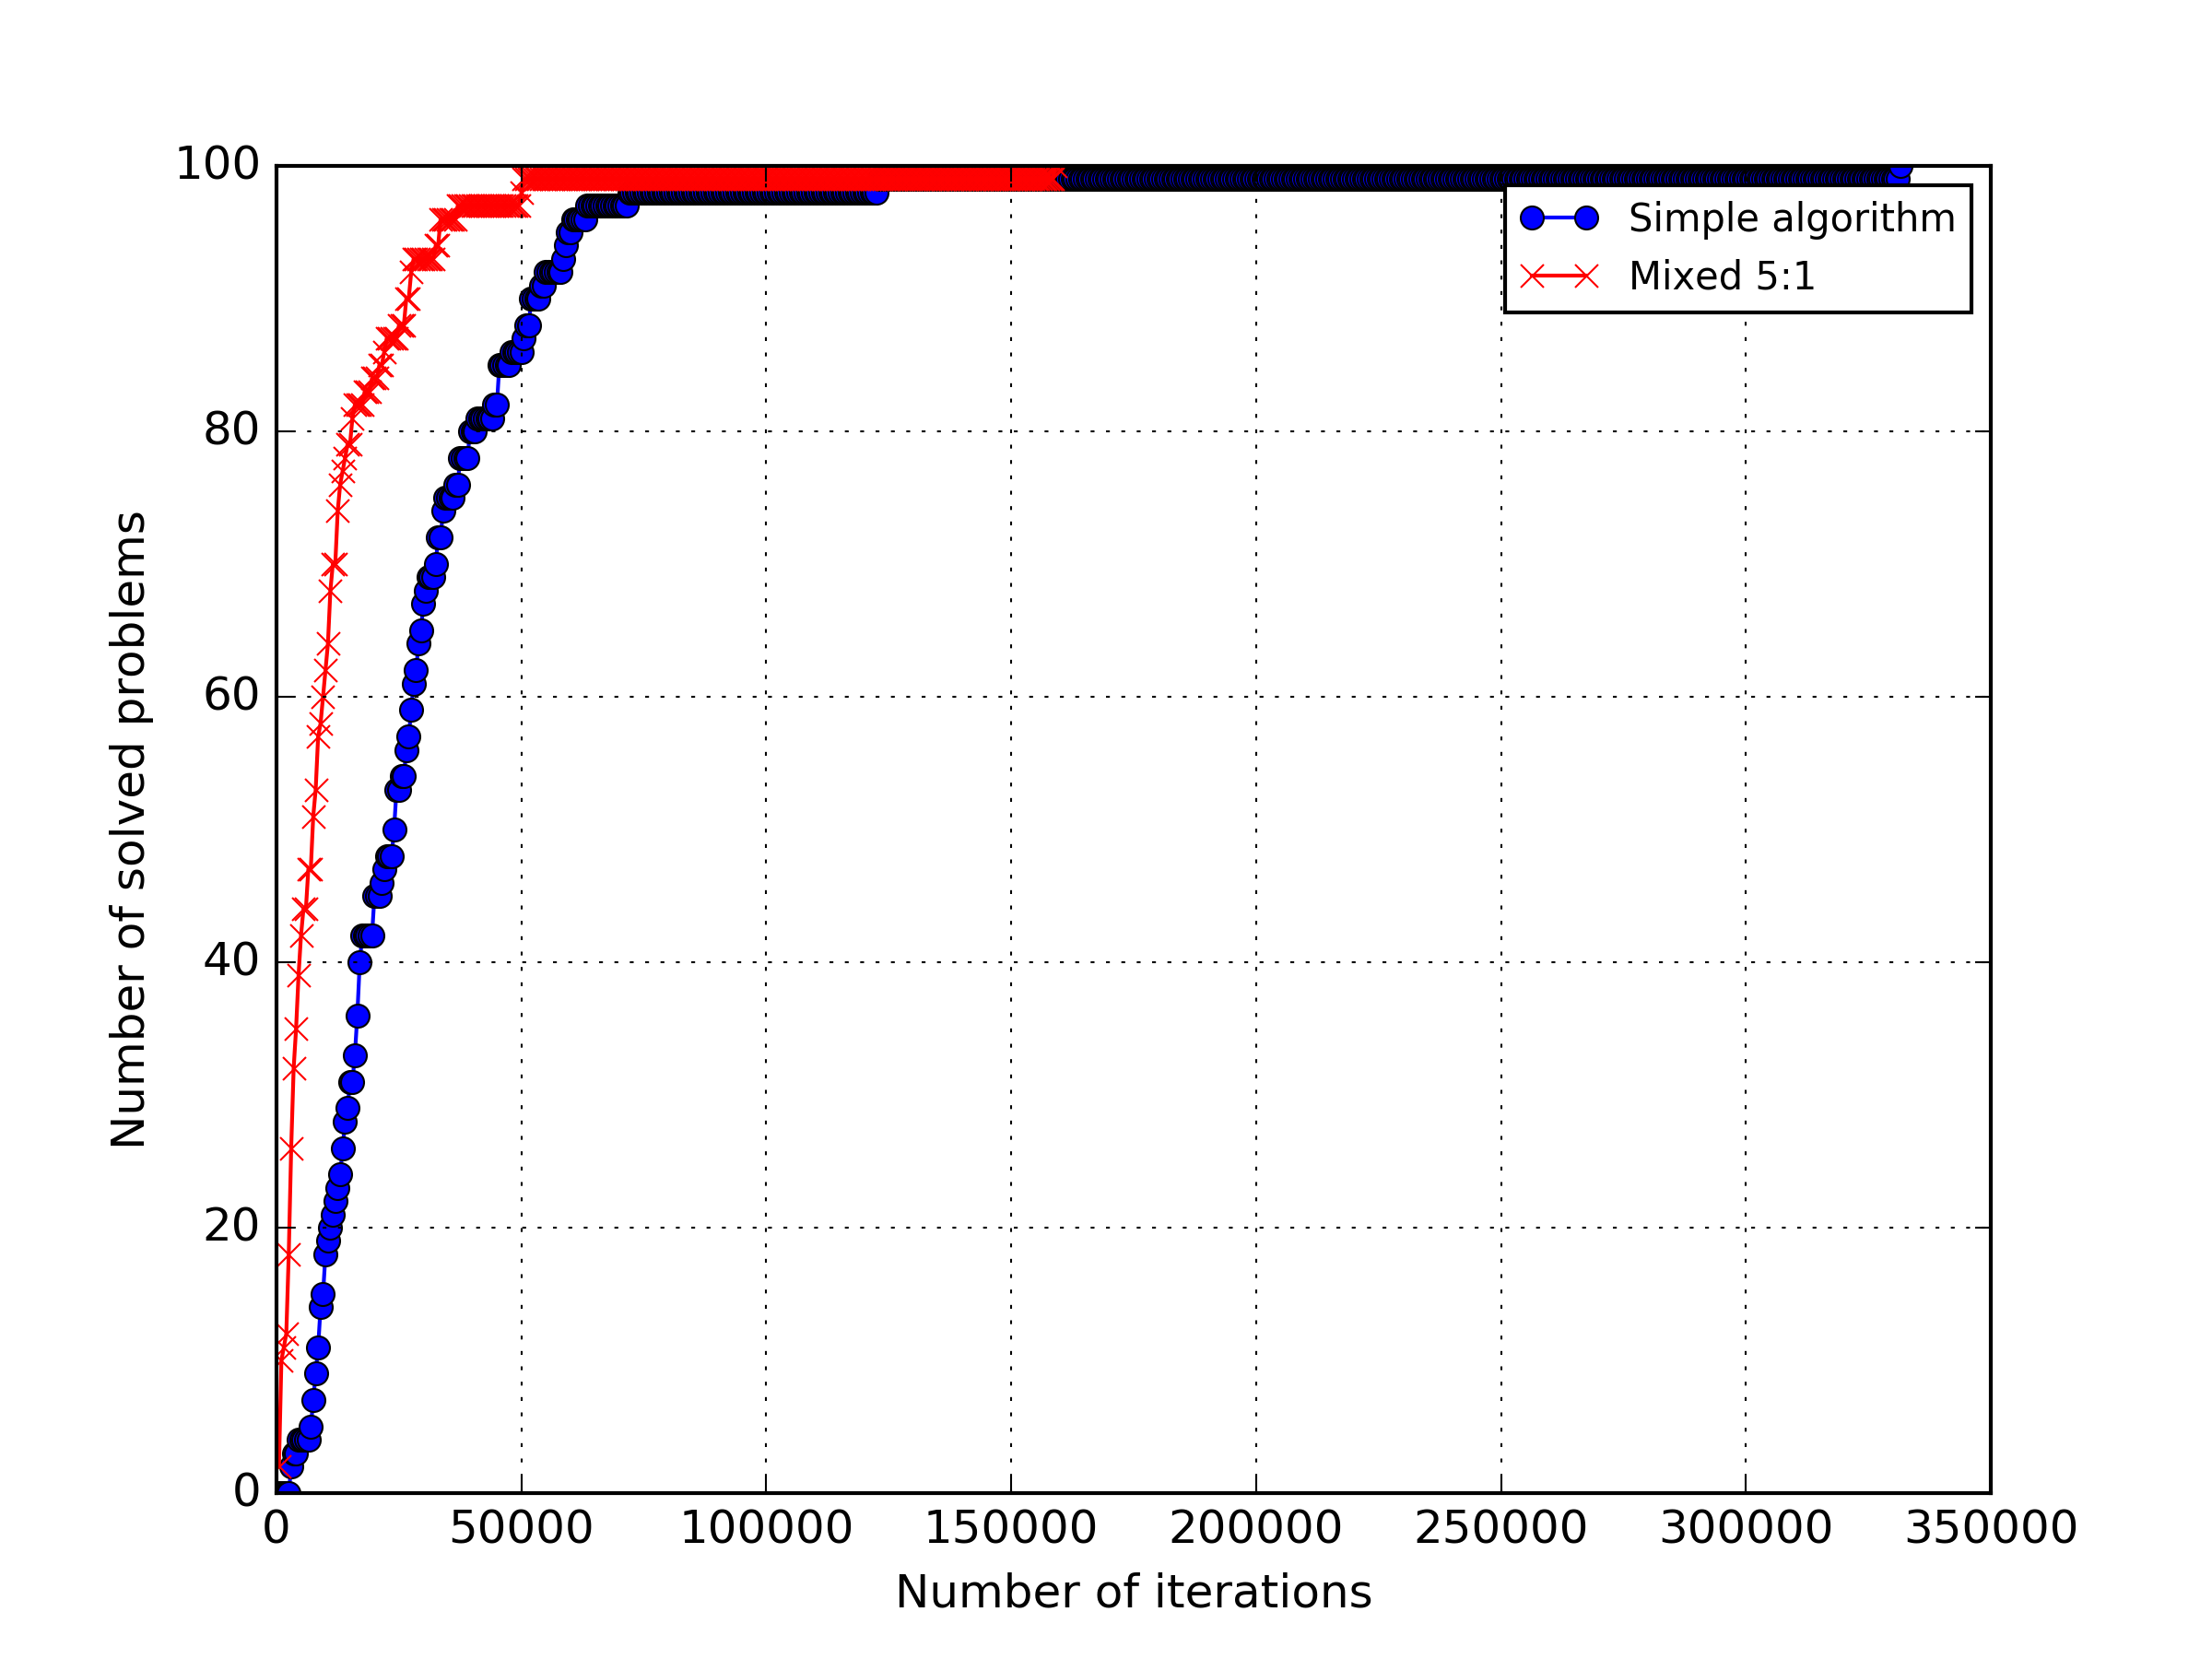
\includegraphics[width=0.75\textwidth]{pictures/mixed_op4d.png}
  \caption{Операционные характеристики на классе GKLS 4d Simple обычного и смешанного АГП}
  \label{fig:localMixOP4d}
\end{figure}
\par
Из-за того, что интервал имеет сразу две характеристики, появляется проблема эффективной реализации смешанного алгоритма. Если интервал имеет одну характеристику, то для выбора максимальной
достаточно организовать очередь характеристик.
Причём, перезаполнение такой очереди необходимо не на каждой итерации: в большинстве случаев характеристики интервалов не меняются, достаточно удалить разбиваемый интервал и вставить в очередь два новых.
Такая организация работы метода озволяет существенно сократить объём вычислений. При наличии у интервала двух характеристик можно организовать две связанные очереди. Рассмотрим этот подход подробнее.
